\documentclass[12pt,a4paper]{article}
\usepackage[utf8]{inputenc}
\usepackage[T1]{fontenc}
\usepackage[english]{babel}
\usepackage{lmodern}
\usepackage{amsmath}
\usepackage{amssymb}
\usepackage{physics}
\usepackage{tcolorbox}
\usepackage{booktabs}
\usepackage{enumitem}
\usepackage[table,xcdraw]{xcolor}
\usepackage[left=2cm,right=2cm,top=2cm,bottom=2cm]{geometry}
\usepackage{pgfplots}
\pgfplotsset{compat=1.18}
\usepackage{graphicx}
\usepackage{float}
\usepackage{fancyhdr}
\usepackage{siunitx}
\usepackage{tikz}
\usepackage{adjustbox}
\usetikzlibrary{shapes.geometric}
\usepackage{hyperref}

% Custom Commands
\newcommand{\Tfield}{T(x)}
\newcommand{\alphaEM}{\alpha_{\text{EM}}}
\newcommand{\betaT}{\beta_{\text{T}}}
\newcommand{\Mpl}{M_{\text{Pl}}}
\newcommand{\Tzerot}{T_0(\Tfield)}
\newcommand{\e}{\mathrm{e}}
\newcommand{\alphaEMSI}{\alpha_{\text{EM,SI}}}
\newcommand{\tablescale}{0.9}

% Header and Footer Configuration
\pagestyle{fancy}
\fancyhf{}
\fancyhead[L]{Johann Pascher}
\fancyhead[R]{Hierarchical Compilation of Units in the T0 Model}
\fancyfoot[C]{\thepage}
\renewcommand{\headrulewidth}{0.4pt}
\renewcommand{\footrulewidth}{0.4pt}

\hypersetup{
	colorlinks=true,
	linkcolor=blue,
	citecolor=blue,
	urlcolor=blue,
	pdftitle={Hierarchical Compilation of Units in the T0 Model with Energy as the Base Unit},
	pdfauthor={Johann Pascher},
	pdfsubject={Theoretical Physics},
	pdfkeywords={T0 Model, natural units, fine-structure constant, unified unit system, time-mass duality}
}

\begin{document}
	
	\title{Hierarchical Compilation of Units in the T0 Model with Energy as the Base Unit}
	\author{Johann Pascher}
	\date{April 13, 2025}
	
	\maketitle
	
	\begin{abstract}
		This work presents a comprehensive hierarchical compilation of natural units within the T0 model of time-mass duality, adopting energy as the fundamental unit. By normalizing dimensional constants (\(\hbar = c = G = k_B = 1\)) and dimensionless coupling constants (\(\alpha_{\text{EM}} = \alpha_W = \beta_T = 1\)) to unity, a unified framework emerges that integrates quantum, relativistic, and cosmological phenomena. The compilation details the hierarchy of constants, quantized length scales from sub-Planckian to cosmic regimes, and the unique presence of biological structures in forbidden zones. Electromagnetic, thermodynamic, and quantum mechanical constants are derived from the energy scale, with simplified field equations revealing the intrinsic unity of natural laws. The Einstein-Hilbert action underpins emergent gravitation, while precise conversions to SI units, philosophical implications, and experimental prospects enrich the discourse. Supported by extensive theoretical derivations and visualizations, this work offers a robust foundation for the T0 model, potentially advancing the unification of physics \cite{pascher_alphabeta_2025}.
	\end{abstract}
	
	\tableofcontents
	\newpage
	
	\section{Introduction}
	\label{sec:introduction}
	
	Natural units streamline physical laws by reducing independent dimensions and setting fundamental constants to unity. The T0 model adopts energy \([E]\) as the base unit, with length and time \([E^{-1}]\), mass and temperature \([E]\), and charge dimensionless. Dimensional constants (\(\hbar = c = G = k_B = 1\)) and dimensionless constants (\(\alpha_{\text{EM}} = \alpha_W = \beta_T = 1\)) are normalized, reflecting a unified framework \cite{pascher_zeit_2025}.
	
	The intrinsic time field is:
	\[
	\Tfield = \frac{\hbar}{\max(m c^2, \omega)}, \quad [\Tfield] = [E^{-1}]
	\]
	It satisfies:
	\[
	\nabla^2 \Tfield = -\kappa \rho(x) \Tfield^2^2, \quad [\kappa] = [E], \quad [\rho] = [E^2]
	\]
	Key parameters:
	\[
	\lambda_0 = m_h \approx \SI{125}{\giga\electronvolt}, \quad [\lambda_0] = [E]
	\]
	\[
	r_g = \frac{GM}{c^2} \text{ (in SI units), which becomes } \frac{M}{M_P^2} \text{ in natural units}, \quad [r_g] = [E^{-1}]
	\]
	These ensure dimensional consistency across scales, as detailed in Sections \ref{sec:hierarchy} and \ref{sec:length_scales}.
	
	\section{Part 1: Overview of Units and Scales}
	\label{sec:hierarchy}
	
	\subsection{Level 1: Primary Dimensional Constants}
	\label{subsec:level1}
	
	The T0 model sets:
	\begin{itemize}
		\item \textbf{Reduced Planck Constant} (\(\hbar = 1\)): \([E^2]\), quantum scale.
		\item \textbf{Speed of Light} (\(c = 1\)): \([E^0]\), relativistic scale.
		\item \textbf{Gravitational Constant} (\(G = 1\)): \([E^{-2}]\), gravitational scale.
		\item \textbf{Boltzmann Constant} (\(k_B = 1\)): \([E^0]\), thermodynamic scale.
	\end{itemize}
	
	Dimensionless constants:
	\begin{itemize}
		\item \textbf{Fine-Structure Constant} (\(\alpha_{\text{EM}} = 1\)): \([E^0]\), SI \(\approx 1/137.036\).
		\item \textbf{Wien’s Constant} (\(\alpha_W = 1\)): \([E^0]\), SI \(\approx 2.82\).
		\item \textbf{T0 Parameter} (\(\beta_T^{\text{nat}} = \frac{\lambda_h^2 v^2}{16\pi^3 m_h^2 \xi} =\tablescale\textwidth}
			\begin{tabular}{lllllll}
				\toprule
				\textbf{Constant} & \textbf{Symbol} & \textbf{SI Value} & \textbf{Natural Value} & \textbf{Dimension} & \textbf{Derivation} & \textbf{Hierarchy Level} \\
				\midrule
				Reduced Planck Constant & \(\hbar\) & \(\SI{1.055e-34}{\joule\second}\) & 1 & \([E^2]\) & Primary & Level 1 \\
				Speed of Light & \(c\) & \(\SI{3e8}{\meter\per\second}\) & 1 & \([E^0]\) & Primary & Level 1 \\
				Gravitational Constant & \(G\) & \(\SI{6.674e-11}{\meter\cubed\per\kilogram\per\second\squared}\) & 1 & \([E^{-2}]\) & Primary & Level 1 \\
				Boltzmann Constant & \(k_B\) & \(\SI{1.381e-23}{\joule\per\kelvin}\) & 1 & \([E^0]\) & Primary & Level 1 \\
				Fine-Structure Constant & \(\alpha_{\text{EM}}\) & 1/137.036 & 1 & \([E^0]\) & Secondary & Level 2 \\
				Wien’s Constant & \(\alpha_W\) & 2.82 & 1 & \([E^0]\) & Secondary & Level 2 \\
				T0 Parameter & \(\beta_T^{\text{nat}}\) & 0.008 & 1 & \([E^0]\) & Secondary & Level 2 \\
				\bottomrule
			\end{tabular}
		\end{adjustbox}
		\caption{Fundamental Constants in the T0 Model}
		\label{tab:fund_const}
	\end{table}
	
	\subsection{Level 2.5: Derived Electromagnetic and Gravitational Constants}
	\label{subsec:level2.5}
	
	Derived constants:
	\begin{itemize}
		\item \textbf{Vacuum Permeability} (\(\mu_0 = 1\)): \([E^0]\), from \(\mu_0 = 1/(\varepsilon_0 c^2)\).
		\item \textbf{Vacuum Permittivity} (\(\varepsilon_0 = 1\)): \([E^0]\), from \(\varepsilon_0 = 1/(\mu_0 c^2)\).
		\item \textbf{Vacuum Impedance} (\(Z_0 = 1\)): \([E^0]\), from \(Z_0 = \sqrt{\mu_0/\varepsilon_0}\).
		\item \textbf{Elementary Charge} (\(e = \sqrt{4\pi} \approx 3.544\)): \([E^0]\), from \(\alpha_{\text{EM}} = e^2/(4\pi \varepsilon_0 \hbar c) = 1\).
		\item \textbf{Coupling Constant} (\(\kappa^{\text{nat}} = \beta_T^{\text{nat}} \cdot \frac{y v}{r_g^2}\)): \([E]\), with \(y = 1/m_h^2 \sim [E^{-2}]\), \(v \sim [E]\), \(r_g \sim [E^{-1}]\).
	\end{itemize}
	
	\textbf{Connection to \(\beta_T\)}:
	\[
	\mu_0 = \varepsilon_0 = 1, \quad \mu_0 \varepsilon_0 = \frac{1}{c^2} = 1
	\]
	\[
	\beta_T^{\text{nat}} = \frac{\lambda_h^2 v^2}{16\pi^3 m_h^2 \xi} = 1, \quad \xi \approx 1.33 \times 10^{-4}
	\]
	This unifies electromagnetic and T0 interactions, independent of standard cosmological assumptions.
	
	\begin{table}[htbp]
		\centering
		\begin{adjustbox}{width=\tablescale\textwidth}
			\begin{tabular}{llllll}
				\toprule
				\textbf{Constant} & \textbf{Symbol} & \textbf{SI Value} & \textbf{Natural Value} & \textbf{Dimension} & \textbf{Hierarchy Level} \\
				\midrule
				Vacuum Permeability & \(\mu_0\) & \(\SI{1.256637061e-6}{\henry\per\meter}\) & 1 & \([E^0]\) & Level 2.5 \\
				Vacuum Permittivity & \(\varepsilon_0\) & \(\SI{8.85e-12}{\farad\per\meter}\) & 1 & \([E^0]\) & Level 2.5 \\
				Vacuum Impedance & \(Z_0\) & \(\SI{376.73}{\ohm}\) & 1 & \([E^0]\) & Level 2.5 \\
				Elementary Charge & \(e\) & \(\SI{1.602e-19}{\coulomb}\) & \(\sqrt{4\pi} \approx 3.544\) & \([E^0]\) & Level 2.5 \\
				Coupling Constant & \(\kappa^{\text{nat}}\) & \(\SI{4.8e-11}{\meter\per\second\squared}\) & \(\beta_T^{\text{nat}} \cdot \frac{y v}{r_g^2}\) & \([E]\) & Level 2.5 \\
				\bottomrule
			\end{tabular}
		\end{adjustbox}
		\caption{Derived Constants}
		\label{tab:em_const}
	\end{table}
	
	\subsection{Planck Units in the T0 Model}
	\label{subsec:planck_units}
	
	\begin{table}[htbp]
		\centering
		\begin{adjustbox}{width=\tablescale\textwidth}
			\begin{tabular}{lcccll}
				\toprule
				\textbf{Planck Unit} & \textbf{Symbol} & \textbf{Definition} & \textbf{SI Value} & \textbf{T0 Dimension} & \textbf{Significance} \\
				\midrule
				Planck Length & \(l_P\) & \(\sqrt{\hbar G/c^3}\) & \(\SI{1.616e-35}{\meter}\) & \([E^{-1}]\) & Length unit \\
				Planck Time & \(t_P\) & \(\sqrt{\hbar G/c^5}\) & \(\SI{5.391e-44}{\second}\) & \([E^{-1}]\) & Time unit \\
				Planck Mass & \(m_P\) & \(\sqrt{\hbar c/G}\) & \(\SI{2.176e-8}{\kilogram}\) & \([E]\) & Mass unit \\
				Planck Energy & \(E_P\) & \(\sqrt{\hbar c^5/G}\) & \(\SI{1.956e9}{\joule}\) & \([E]\) & Energy unit \\
				Planck Temperature & \(T_P\) & \(\sqrt{\hbar c^5/G}/k_B\) & \(\SI{1.417e32}{\kelvin}\) & \([E]\) & Temperature unit \\
				Planck Charge & \(q_P\) & \(\sqrt{4\pi \varepsilon_0 \hbar c}\) & \(\SI{1.875e-18}{\coulomb}\) & \([E^0]\) & Charge unit \\
				Planck Pressure & \(p_P\) & \(c^7/(\hbar G^2)\) & \(\SI{4.633e113}{\pascal}\) & \([E^4]\) & Pressure unit \\
				Planck Density & \(\rho_P\) & \(c^5/(\hbar G^2)\) & \(\SI{5.155e96}{\kilogram\per\meter\cubed}\) & \([E^4]\) & Density unit \\
				\bottomrule
			\end{tabular}
		\end{adjustbox}
		\caption{Planck Units in the T0 Model}
		\label{tab:planck_units}
	\end{table}
	
	\subsection{Characteristic Length Scales}
	\label{sec:length_scales}
	
	Length scales span 97 orders of magnitude, derived from model-internal parameters:
	
	\begin{table}[H]
		\centering
		\begin{adjustbox}{width=\tablescale\textwidth}
			\begin{tabular}{lcccc}
				\toprule
				\textbf{Structure} & \textbf{With \(l_P = 1\)} & \textbf{With \(r_0 = 1\)} & \textbf{Dimension} & \textbf{Relationship} \\
				\midrule
				Planck Length (\(l_P\)) & 1 & \(1/\xi \approx 7519\) & \([E^{-1}]\) & Base unit \\
				T0 Length (\(r_0\)) & \(\xi \approx 1.33 \times 10^{-4}\) & 1 & \([E^{-1}]\) & \(\xi \cdot l_P\) \\
				Strong Scale & \(\sim 10^{-19}\) & \(\sim 10^{-15}\) & \([E^{-1}]\) & \(\sim \alpha_s \cdot \lambda_{C,h}\) \\
				Higgs Length (\(\lambda_{C,h}\)) & \(\sim 1.6 \times 10^{-20}\) & \(\sim 1.2 \times 10^{-16}\) & \([E^{-1}]\) & \(m_P/m_h \cdot l_P\) \\
				Proton Radius & \(\sim 5.2 \times 10^{-20}\) & \(\sim 3.9 \times 10^{-16}\) & \([E^{-1}]\) & \(\sim \alpha_s/(2\pi) \cdot \lambda_{C,p}\) \\
				Electron Radius (\(r_e\)) & \(\sim 2.4 \times 10^{-23}\) & \(\sim 1.8 \times 10^{-19}\) & \([E^{-1}]\) & \(\alpha_{\text{EM,SI}}/(2\pi) \cdot \lambda_{C,e}\) \\
				Compton Length (\(\lambda_{C,e}\)) & \(\sim 2.1 \times 10^{-23}\) & \(\sim 1.6 \times 10^{-19}\) & \([E^{-1}]\) & \(m_P/m_e \cdot l_P\) \\
				Bohr Radius (\(a_0\)) & \(\sim 2.9 \times 10^{-21}\) & \(\sim 2.2 \times 10^{-17}\) & \([E^{-1}]\) & \(\lambda_{C,e}/\alpha_{\text{EM,SI}}\) \\
				DNA Width & \(\sim 1.2 \times 10^{-26}\) & \(\sim 9.0 \times 10^{-23}\) & \([E^{-1}]\) & \(\sim \lambda_{C,e} \cdot m_e/m_{\text{DNA}}\) \\
				Cell & \(\sim 6.2 \times 10^{-30}\) & \(\sim 4.7 \times 10^{-26}\) & \([E^{-1}]\) & \(\sim 10^7 \cdot \text{DNA}\) \\
				Human & \(\sim 6.2 \times 10^{-35}\) & \(\sim 4.7 \times 10^{-31}\) & \([E^{-1}]\) & \(\sim 10^5 \cdot \text{Cell}\) \\
				Earth Radius & \(\sim 3.9 \times 10^{-41}\) & \(\sim 2.9 \times 10^{-37}\) & \([E^{-1}]\) & \(\sim (m_P/m_{\text{Earth}})^2 \cdot l_P\) \\
				Sun Radius & \(\sim 4.3 \times 10^{-43}\) & \(\sim 3.2 \times 10^{-39}\) & \([E^{-1}]\) & \(\sim (m_P/m_{\text{Sun}})^2 \cdot l_P\) \\
				Solar System & \(\sim 6.2 \times 10^{-47}\) & \(\sim 4.7 \times 10^{-43}\) & \([E^{-1}]\) & \(\sim \alpha_G^{-1/2} \cdot \text{Sun}\) \\
				Galaxy & \(\sim 6.2 \times 10^{-56}\) & \(\sim 4.7 \times 10^{-52}\) & \([E^{-1}]\) & \(\sim (m_P/m_{\text{Galaxy}})^2 \cdot l_P\) \\
				Cluster & \(\sim 6.2 \times 10^{-58}\) & \(\sim 4.7 \times 10^{-54}\) & \([E^{-1}]\) & \(\sim 10^2 \cdot \text{Galaxy}\) \\
				Correlation Length (\(L_T\)) & \(\sim 3.9 \times 10^{62}\) & \(\sim 2.9 \times 10^{66}\) & \([E^{-1}]\) & \(\beta_T^{\text{nat}}{}^{-1/4} \cdot \xi^{-1/2} \cdot l_P\) \\
				\bottomrule
			\end{tabular}
		\end{adjustbox}
		\caption{Length Scales in the T0 Model, derived from model-internal parameters}
		\label{tab:length_scales}
	\end{table}
	
	\textbf{Note}: The correlation length \(L_T\) is derived from \(\beta_T^{\text{nat}}\) and \(\xi\), based on Higgs parameters, independent of standard cosmological constants like \(H_0\).
	
	\begin{figure}[htbp]
		\centering
		\begin{tikzpicture}
			\small
			\draw[thick,->] (0,0) -- (12,0) node[right] {$\log(L/l_P)$};
			\draw[thick,->] (0,0) -- (0,5) node[above] {Energy Scale};
			\draw (0,0.2) -- (0,-0.2) node[below] {$0$};
			\draw (1,0.2) -- (1,-0.2) node[below] {$r_0$};
			\draw (5,0.2) -- (5,-0.2) node[below] {$\lambda_{C,e}$};
			\draw (6,0.2) -- (6,-0.2) node[below] {$a_0$};
			\draw (11,0.2) -- (11,-0.2) node[below] {$L_T$};
			\node[blue] at (0,1.2) {$l_P = 1$};
			\node[blue] at (1,1.7) {$r_0 \approx 10^{-4}$};
			\node[blue] at (5,1.7) {$\lambda_{C,e} \approx 10^{-23}$};
			\node[blue] at (6,1.2) {$a_0 \approx 2.9 \times 10^{-21}$};
			\node[blue] at (11,1.2) {$L_T \approx 10^{62}$};
			\draw [decorate,decoration={brace,amplitude=10pt,mirror},xshift=0pt,yshift=-20pt]
			(0,0) -- (1,0) node [black,midway,yshift=-20pt] {Primordial Scale};
			\draw [decorate,decoration={brace,amplitude=10pt,mirror},xshift=0pt,yshift=-20pt]
			(4.8,0) -- (6.2,0) node [black,midway,yshift=-20pt] {Quantum Scale};
			\draw [decorate,decoration={brace,amplitude=10pt,mirror},xshift=0pt,yshift=-20pt]
			(10.8,0) -- (12,0) node [black,midway,yshift=-20pt] {Cosmological Scale};
			\draw[dashed, red] (1,0.5) -- (5,0.5) node[midway, above] {$\propto m_h/m_e$};
		\end{tikzpicture}
		\caption{Hierarchy of Length Scales}
		\label{fig:length_hierarchy}
	\end{figure}
	
	\subsection{Biological Anomalies in Forbidden Zones}
	\label{sec:bio_anomalies}
	
	Biological structures occupy forbidden zones:
	\[
	\nabla^2 \Tfield_{\text{bio}} \approx -\kappa \rho(x) \Tfield_{\text{bio}}^2 + \delta_{\text{bio}}(x,t), \quad [\kappa] = [E]
	\]
	
	\begin{table}[htbp]
		\centering
		\begin{adjustbox}{width=\tablescale\textwidth}
			\begin{tabular}{lccc}
				\toprule
				\textbf{Structure} & \textbf{Size} & \textbf{Ratio to \(l_P\)} & \textbf{Position} \\
				\midrule
				DNA Diameter & \(\SI{2e-9}{\meter}\) & \(\sim 10^{-26}\) & Forbidden Zone \\
				Protein & \(\SI{1e-8}{\meter}\) & \(\sim 10^{-27}\) & Forbidden Zone \\
				Bacterium & \(\SI{1e-6}{\meter}\) & \(\sim 10^{-29}\) & Forbidden Zone \\
				Cell & \(\SI{1e-5}{\meter}\) & \(\sim 10^{-30}\) & Forbidden Zone \\
				Organism & \(\SIrange{1e-3}{1}{\meter}\) & \(\sim 10^{-32} - 10^{-35}\) & Forbidden Zone \\
				\bottomrule
			\end{tabular}
		\end{adjustbox}
		\caption{Biological Structures in Forbidden Zones}
		\label{tab:bio_anomalies}
	\end{table}
	
	\begin{figure}[htbp]
		\centering
		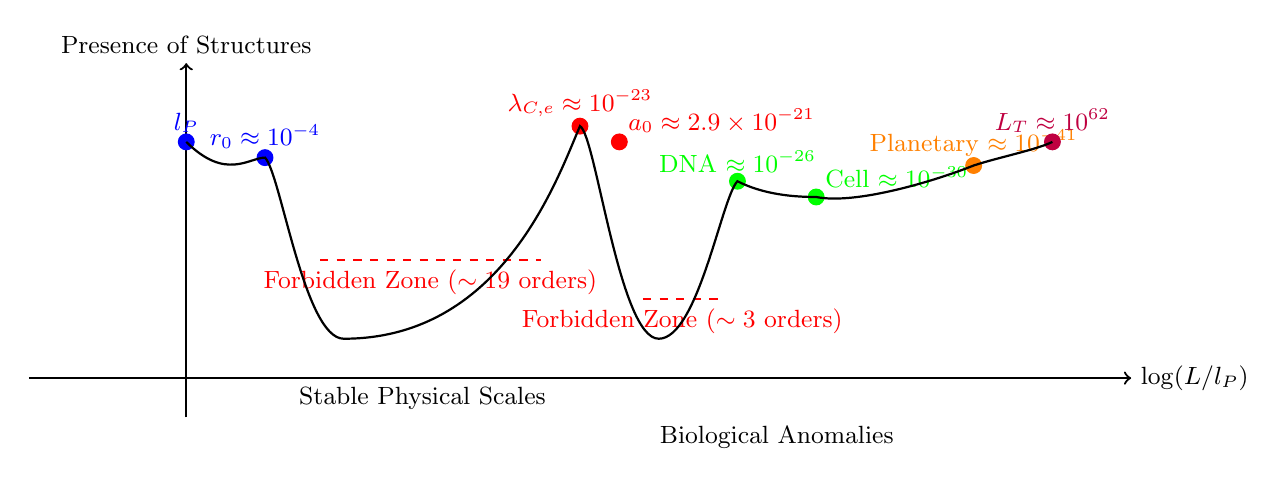
\begin{tikzpicture}
			\small
			\draw[thick,->] (-2,0) -- (12,0) node[right] {$\log(L/l_P)$};
			\draw[thick,->] (0,-0.5) -- (0,4) node[above] {Presence of Structures};
			\filldraw[blue] (0,3) circle (0.1) node[above] {$l_P$};
			\filldraw[blue] (1,2.8) circle (0.1) node[above] {$r_0 \approx 10^{-4}$};
			\filldraw[red] (5,3.2) circle (0.1) node[above] {$\lambda_{C,e} \approx 10^{-23}$};
			\filldraw[red] (5.5,3) circle (0.1) node[above right] {$a_0 \approx 2.9 \times 10^{-21}$};
			\filldraw[green] (7,2.5) circle (0.1) node[above] {DNA $\approx 10^{-26}$};
			\filldraw[green] (8,2.3) circle (0.1) node[above right] {Cell $\approx 10^{-30}$};
			\filldraw[orange] (10,2.7) circle (0.1) node[above] {Planetary $\approx 10^{-41}$};
			\filldraw[purple] (11,3) circle (0.1) node[above] {$L_T \approx 10^{62}$};
			\draw[thick, dashed, red] (1.7,1.5) -- (4.5,1.5) node[midway, below] {Forbidden Zone ($\sim 19$ orders)};
			\draw[thick, dashed, red] (5.8,1) -- (6.8,1) node[midway, below] {Forbidden Zone ($\sim 3$ orders)};
			\draw[smooth, thick] (0,3) .. controls (0.5,2.5) and (0.8,2.8) .. (1,2.8)
			.. controls (1.2,2.6) and (1.5,0.5) .. (2,0.5)
			.. controls (4,0.5) and (4.7,2.5) .. (5,3.2)
			.. controls (5.2,3.1) and (5.5,0.5) .. (6,0.5)
			.. controls (6.5,0.5) and (6.8,2.3) .. (7,2.5)
			.. controls (7.2,2.4) and (7.5,2.3) .. (8,2.3)
			.. controls (8.5,2.2) and (9.5,2.5) .. (10,2.7)
			.. controls (10.3,2.8) and (10.8,2.9) .. (11,3);
			\node[align=center, below] at (3,0) {Stable Physical Scales};
			\node[align=center, below] at (7.5,-0.5) {Biological Anomalies};
		\end{tikzpicture}
		\caption{Stability Centers and Forbidden Zones}
		\label{fig:stability_zones}
	\end{figure}
	
	\section{Part 2: Detailed Explanations and Derivations}
	\label{sec:derivations}
	
	\subsection{Fundamental Concepts of the T0 Model}
	\label{subsec:concepts}
	
	The T0 model posits absolute time and variable mass, with:
	\[
	\Tfield = \frac{\hbar}{\max(m c^2, \omega)}, \quad \nabla^2 \Tfield = -\kappa \rho(x) \Tfield^2^2
	\]
	Energy unifies quantities: mass, temperature \([E]\); length, time \([E^{-1}]\).
	
	\subsection{Derivation of \(\beta_T^{\text{nat}} = \frac{\lambda_h^2 v^2}{16\pi^3 m_h^2 \xi} = \frac{\lambda_h^2 v^2}{16 \pi^3 m_h^2 \xi}
	\]
	Parameters:
	\begin{itemize}
		\item \(\lambda_h \approx 0.13\): Higgs self-coupling, \([E^0]\).
		\item \(v \approx \SI{246}{\giga\electronvolt}\): Higgs vacuum expectation value, \([E]\).
		\item \(m_h \approx \SI{125}{\giga\electronvolt}\): Higgs mass, \([E]\).
		\item \(\xi \approx 1.33 \times 10^{-4}\): Scaling factor for the T0 length, defined as:
		\[
		\xi = \frac{\lambda_h^2 v^2}{16 \pi^3 m_h^2}, \quad r_0 = \xi \cdot l_P
		\]
	\end{itemize}
	\textbf{Note}: The values of \(\lambda_h\), \(v\), and \(m_h\) are derived from SI units, based on experimental measurements from the Standard Model.
	\[
	\beta_T^{\text{nat}} = \frac{\lambda_h^2 v^2}{16\pi^3 m_h^2 \xi} = 1
	\]
	\[
	[\beta_T^{\text{nat}}] = [E^0]
	\]
	\[
	r_0 = \xi \cdot l_P, \quad [r_0] = [E^{-1}]
	\]
	
	\textbf{Electromagnetic Derivation}:
	The T0 model unifies fundamental interactions by normalizing coupling constants to 1. The fine-structure constant is set as:
	\[
	\alpha_{\text{EM}} = \frac{e^2}{4 \pi \varepsilon_0 \hbar c} = 1 \implies e = \sqrt{4 \pi}, \quad \varepsilon_0 = \mu_0 = 1
	\]
	Similarly, the T0 parameter is normalized to \(\beta_T^{\text{nat}} = \frac{\lambda_h^2 v^2}{16\pi^3 m_h^2 \xi} = 1\)}
	\label{subsec:alpha_derivation}
	
	\[
	\alpha_{\text{EM}} = \frac{e^2}{4 \pi \varepsilon_0 \hbar c} = 1 \implies e = \sqrt{4 \pi}
	\]
	\[
	[\alpha_{\text{EM}}] = [E^0]
	\]
	\[
	\text{Note: } \alpha^{\text{nat}} = \lambda_h^2 v / L_T^2 \text{ is not used, as it yields } [E^3].
	\]
	
	\subsection{Connection to Higgs Parameters}
	\label{subsec:higgs}
	
	\[
	r_0 = \xi \cdot l_P, \quad \xi \approx 1.33 \times 10^{-4}, \quad [r_0] = [E^{-1}]
	\]
	
	\subsection{Quantization of Length Scales}
	\label{subsec:quantization}
	
	\[
	L_n = l_P \times \prod_i \alpha_i^{n_i}, \quad \alpha_i = \{\alpha_{\text{EM}}, \beta_T^{\text{nat}}, \xi\}
	\]
	
	\begin{figure}[htbp]
		\centering
		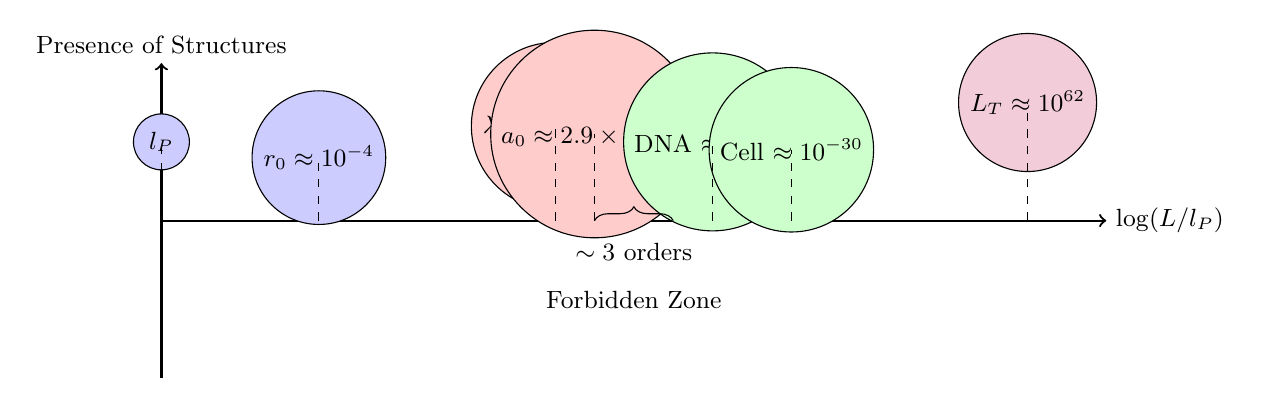
\begin{tikzpicture}
			\small
			\draw[thick,->] (0,0) -- (12,0) node[right] {$\log(L/l_P)$};
			\draw[thick,->] (0,-2) -- (0,2) node[above] {Presence of Structures};
			\node at (0,1) [circle, draw, fill=blue!20] {$l_P$};
			\node at (2,0.8) [circle, draw, fill=blue!20] {$r_0 \approx 10^{-4}$};
			\node at (5,1.2) [circle, draw, fill=red!20] {$\lambda_{C,e} \approx 10^{-23}$};
			\node at (5.5,1.1) [circle, draw, fill=red!20] {$a_0 \approx 2.9 \times 10^{-21}$};
			\node at (7,1) [circle, draw, fill=green!20] {DNA $\approx 10^{-26}$};
			\node at (8,0.9) [circle, draw, fill=green!20] {Cell $\approx 10^{-30}$};
			\node at (11,1.5) [circle, draw, fill=purple!20] {$L_T \approx 10^{62}$};
			\draw[dashed] (0,0) -- (0,1);
			\draw[dashed] (2,0) -- (2,0.8);
			\draw[dashed] (5,0) -- (5,1.2);
			\draw[dashed] (5.5,0) -- (5.5,1.1);
			\draw[dashed] (7,0) -- (7,1);
			\draw[dashed] (8,0) -- (8,0.9);
			\draw[dashed] (11,0) -- (11,1.5);
			\node at (6,-1) {Forbidden Zone};
			\draw[decorate,decoration={brace,amplitude=5pt}] (5.5,0) -- (6.5,0) node[midway,below,yshift=-5pt] {$\sim 3$ orders};
		\end{tikzpicture}
		\caption{Analogy to Atomic Orbitals}
		\label{fig:orbital_analogy}
	\end{figure}
	
	\subsection{Einstein-Hilbert Action and Emergent Gravitation}
	\label{sec:gravitation}
	
	\[
	S_{\text{EH}} = \frac{1}{16 \pi} \int (R - 2 \kappa^{\text{nat}}) \sqrt{-g} \, d^4x
	\]
	\[
	\Phi(r) = -\frac{r_g}{r} + \kappa r + \kappa^{\text{nat}} r, \quad \kappa^{\text{nat}} = \beta_T^{\text{nat}} \cdot \frac{y v}{r_g^2}, \quad [\kappa^{\text{nat}}] = [E]
	\]
	\[
	y = \frac{1}{m_h^2}, \quad \beta_T^{\text{nat}} = \frac{\lambda_h^2 v^2}{16\pi^3 m_h^2 \xi} = -\ln\left(\frac{\Tfield}{\Tfield_0}\right)
	\]
	
	\begin{table}[htbp]
		\centering
		\begin{adjustbox}{width=\tablescale\textwidth}
			\begin{tabular}{p{3cm}p{3cm}p{4cm}p{4cm}}
				\toprule
				\textbf{Theory} & \textbf{Principle} & \textbf{Potential} & \textbf{Comparison with T0} \\
				\midrule
				Newtonian & Force & \(-\frac{G M}{r}\) & T0 special case (\(\kappa^{\text{nat}} = 0\)) \\
				General Relativity & Curvature & Schwarzschild & Equivalent in weak fields \\
				MOND & Modified dynamics & \(\mu(\nabla \Phi/a_0)\) & T0 provides basis \\
				f(R) Theories & Modified action & Varies & T0: f(R) = R - 2\(\kappa^{\text{nat}}\) G \\
				T0 Model & Time field & \(-\frac{r_g}{r} + \kappa^{\text{nat}} r\) & Unifies QM and gravitation \\
				\bottomrule
			\end{tabular}
		\end{adjustbox}
		\caption{Comparison of Gravitation Theories}
		\label{tab:theory_comparison}
	\end{table}
	
	\subsubsection{Equivalence between Einstein-Hilbert Action and Time Field Derivation}
	Both yield:
	\[
	\Phi(r) = -\frac{r_g}{r} + \kappa r + \kappa^{\text{nat}} r, \quad [\kappa^{\text{nat}}] = [E]
	\]
	
	\subsection{Field Equations}
	\label{sec:field_equations}
	
	\subsubsection{Maxwell Equations}
	\label{subsec:maxwell}
	
	\begin{table}[htbp]
		\centering
		\begin{adjustbox}{width=\tablescale\textwidth}
			\begin{tabular}{llll}
				\toprule
				\textbf{Equation} & \textbf{Classical Form} & \textbf{Natural Form} & \textbf{Dimension} \\
				\midrule
				Gauss’s Law & \(\nabla \cdot \vec{E} = \frac{\rho}{\varepsilon_0}\) & \(\nabla \cdot \vec{E} = \rho\) & \([E^2]\) \\
				Ampère’s Law & \(\nabla \times \vec{B} - \mu_0 \varepsilon_0 \frac{\partial \vec{E}}{\partial t} = \mu_0 \vec{j}\) & \(\nabla \times \vec{B} - \frac{\partial \vec{E}}{\partial t} = \vec{j}\) & \([E]\) \\
				Gauss for Magnetism & \(\nabla \cdot \vec{B} = 0\) & \(\nabla \cdot \vec{B} = 0\) & \([E^0]\) \\
				Faraday’s Law & \(\nabla \times \vec{E} + \frac{\partial \vec{B}}{\partial t} = 0\) & \(\nabla \times \vec{E} + \frac{\partial \vec{B}}{\partial t} = 0\) & \([E^0]\) \\
				\bottomrule
			\end{tabular}
		\end{adjustbox}
		\caption{Maxwell Equations in Natural Units}
		\label{tab:maxwell}
	\end{table}
	
	\subsubsection{T0 Model Equations}
	\label{subsec:t0_equations}
	
	\begin{table}[htbp]
		\centering
		\begin{adjustbox}{width=\tablescale\textwidth}
			\begin{tabular}{lll}
				\toprule
				\textbf{Equation} & \textbf{Natural Form} & \textbf{Significance} \\
				\midrule
				Temperature-Redshift & \(T(z) = T_0 (1+z)(1+\ln(1+z))\) & Cosmic temperature \\
				Wavelength Redshift & \(z(\lambda) = z_0 (1+\ln(\lambda/\lambda_0))\) & Frequency-dependent \\
				Gravitational Potential & \(\Phi(r) = -\frac{r_g}{r} + \kappa r + \kappa^{\text{nat}} r\) & Emergent gravitation \\
				Intrinsic Time Field & \(\nabla^2 \Tfield = -\kappa \rho(x) \Tfield^2^2\) & Source term \\
				Effective Potential & \(\Phi(\vec{x}) = -\ln\left(\frac{\Tfield}{\Tfield_0}\right)\) & Gravitation link \\
				Gravitational Force & \(\vec{F} = -\frac{\nabla \Tfield}{\Tfield}\) & Force from time field \\
				\bottomrule
			\end{tabular}
		\end{adjustbox}
		\caption{T0 Model Equations}
		\label{tab:t0_equations}
	\end{table}
	
	\textbf{Note}: Temperature-redshift is consistent with \(\beta_T^{\text{nat}} = \frac{\lambda_h^2 v^2}{16\pi^3 m_h^2 \xi} = 1\).
	
	\subsubsection{Modified Quantum Mechanics}
	\label{subsec:quantum}
	
	\begin{table}[htbp]
		\centering
		\begin{adjustbox}{width=\tablescale\textwidth}
			\begin{tabular}{lll}
				\toprule
				\textbf{Equation} & \textbf{Natural Form} & \textbf{Standard Form} \\
				\midrule
				Schrödinger Equation & \(i \Tfield \frac{\partial \Psi}{\partial t} + i \Psi \frac{\partial \Tfield}{\partial t} = \hat{H} \Psi\) & \(i \hbar \frac{\partial \Psi}{\partial t} = \hat{H} \Psi\) \\
				Decoherence Rate & \(\Gamma_{\text{dec}} = \Gamma_0 \cdot m\) & \(\Gamma_{\text{dec}} = \Gamma_0 \cdot \frac{m c^2}{\hbar}\) \\
				Wave-Particle & \(\lambda = \frac{1}{p}\) & \(\lambda = \frac{h}{p}\) \\
				Uncertainty & \(\Delta E \cdot \Delta t \geq \frac{1}{2}\) & \(\Delta E \cdot \Delta t \geq \frac{\hbar}{2}\) \\
				\bottomrule
			\end{tabular}
		\end{adjustbox}
		\caption{Modified Quantum Equations}
		\label{tab:qm_equations}
	\end{table}
	
	\subsection{Fundamental Relationships}
	\label{subsec:relationships}
	
	\begin{figure}[htbp]
		\centering
		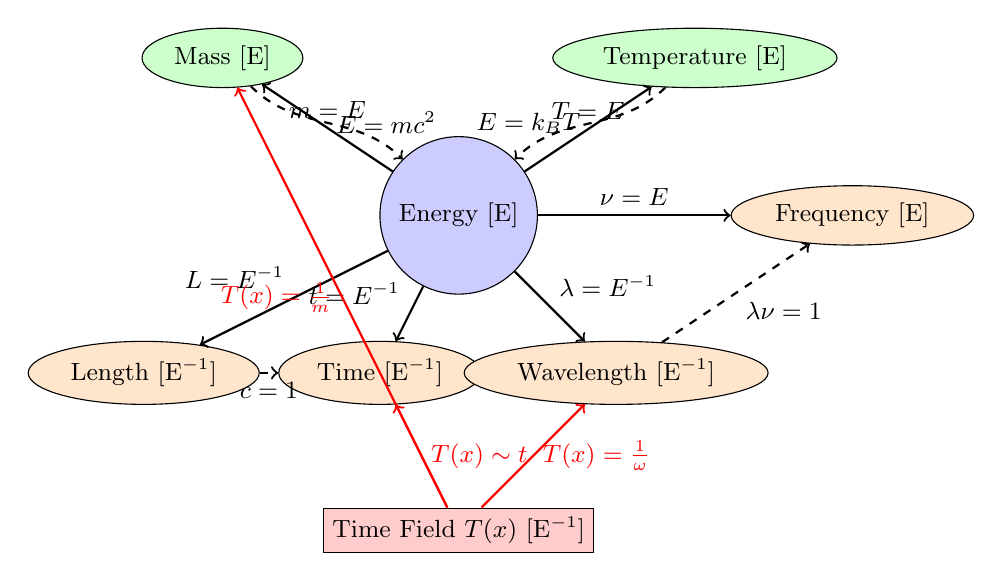
\begin{tikzpicture}
			\small
			\node[draw, circle, fill=blue!20, minimum size=2cm] (energy) at (0,0) {Energy [E]};
			\node[draw, ellipse, fill=green!20] (mass) at (-3,2) {Mass [E]};
			\node[draw, ellipse, fill=green!20] (temp) at (3,2) {Temperature [E]};
			\node[draw, ellipse, fill=orange!20] (length) at (-4,-2) {Length [E\(^{-1}\)]};
			\node[draw, ellipse, fill=orange!20] (time) at (-1,-2) {Time [E\(^{-1}\)]};
			\node[draw, ellipse, fill=orange!20] (wavelength) at (2,-2) {Wavelength [E\(^{-1}\)]};
			\node[draw, ellipse, fill=orange!20] (frequency) at (5,0) {Frequency [E]};
			\node[draw, rectangle, fill=red!20] (tfield) at (0,-4) {Time Field \(\Tfield\) [E\(^{-1}\)]};
			\draw[->, thick] (energy) -- (mass) node[midway, above] {$m = E$};
			\draw[->, thick] (energy) -- (temp) node[midway, above] {$T = E$};
			\draw[->, thick] (energy) -- (length) node[midway, above left] {$L = E^{-1}$};
			\draw[->, thick] (energy) -- (time) node[midway, above left] {$t = E^{-1}$};
			\draw[->, thick] (energy) -- (wavelength) node[midway, above right] {$\lambda = E^{-1}$};
			\draw[->, thick] (energy) -- (frequency) node[midway, above] {$\nu = E$};
			\draw[->, thick, dashed] (length) -- (time) node[midway, below] {$c = 1$};
			\draw[->, thick, dashed] (wavelength) -- (frequency) node[midway, below right] {$\lambda \nu = 1$};
			\draw[->, thick, dashed] (mass) to[out=-45, in=135] node[midway, right] {$E = m c^2$} (energy);
			\draw[->, thick, dashed] (temp) to[out=-135, in=45] node[midway, left] {$E = k_B T$} (energy);
			\draw[->, thick, red] (tfield) -- (mass) node[midway, left] {$\Tfield = \frac{1}{m}$};
			\draw[->, thick, red] (tfield) -- (time) node[midway, right] {$\Tfield \sim t$};
			\draw[->, thick, red] (tfield) -- (wavelength) node[midway, right] {$\Tfield = \frac{1}{\omega}$};
		\end{tikzpicture}
		\caption{Network of Physical Quantities}
		\label{fig:quantity_network}
	\end{figure}
	
	\begin{figure}[htbp]
		\centering
		\begin{tikzpicture}
			\footnotesize
			\draw[thick, ->] (0,0) -- (12,0) node[right] {Energy Scale};
			\draw[thick, ->] (0,0) -- (0,4) node[above] {Mass Range};
			\draw[thick] (2,0.2) -- (2,-0.2) node[below] {Planck};
			\draw[thick] (5,0.2) -- (5,-0.2) node[below] {Electroweak};
			\draw[thick] (8,0.2) -- (8,-0.2) node[below] {QCD};
			\draw[thick] (11,0.2) -- (11,-0.2) node[below] {Atomic};
			\node[draw, fill=blue!10] at (2,2.5) {$M_P \sim \SI{1e19}{\giga\electronvolt}$};
			\node[draw, fill=blue!10] at (5,2) {$M_W, M_Z, M_H \sim \SI{1e2}{\giga\electronvolt}$};
			\node[draw, fill=blue!10] at (8,1.5) {$\Lambda_{QCD} \sim \SI{0.2}{\giga\electronvolt}$};
			\node[draw, fill=blue!10] at (11,1) {$m_e \sim \SI{0.0005}{\giga\electronvolt}$};
			\draw[thick, red, ->] (2,3.5) -- (5,2.5) node[midway, above] {$\xi = 1.33 \times 10^{-4}$};
			\draw[thick, red, ->] (5,2.5) -- (8,2) node[midway, above] {$\alpha_{\text{EM}} = 1$};
			\draw[thick, red, ->] (8,2) -- (11,1.5) node[midway, above] {$\beta_T^{\text{nat}} = \frac{\lambda_h^2 v^2}{16\pi^3 m_h^2 \xi} =red!10] at (6,3.9) {T0 Model: $\hbar = c = G = \alpha_{\text{EM}} = \beta_T^{\text{nat}} = \frac{\lambda_h^2 v^2}{16\pi^3 m_h^2 \xi} =\tablescale\textwidth}
			\begin{tabular}{llll}
				\toprule
				\textbf{Force} & \textbf{Dimensionless Coupling} & \textbf{Natural Value} & \textbf{Range} \\
				\midrule
				Electromagnetic & \(\alpha_{\text{EM}}\) & 1 & \(\infty\) \\
				Strong & \(\alpha_s\) & \(\sim 0.118\) at \(Q^2 = M_Z^2\) & \(\sim \SI{1e-15}{\meter}\) \\
				Weak & \(\alpha_W = g^2/(4\pi)\) & \(\sim 1/30\) & \(\sim \SI{1e-18}{\meter}\) \\
				Gravitation & \(\alpha_G = G m^2/\hbar c\) & \(m^2/m_P^2\) & \(\infty\) \\
				\bottomrule
			\end{tabular}
		\end{adjustbox}
		\caption{Fundamental Forces in Natural Units}
		\label{tab:forces}
	\end{table}
	
	\subsection{Unit Conversions}
	\label{sec:conversions}
	
	\begin{table}[htbp]
		\centering
		\begin{adjustbox}{width=\tablescale\textwidth}
			\begin{tabular}{lcccc}
				\toprule
				\textbf{SI Unit} & \textbf{SI Dimension} & \textbf{T0 Equivalent} & \textbf{Conversion} & \textbf{Accuracy} \\
				\midrule
				Meter & \([L]\) & \([E^{-1}]\) & \(\SI{1}{\meter} \leftrightarrow (\SI{197}{\mega\electronvolt})^{-1}\) & \(< 0.001\%\) \\
				Second & \([T]\) & \([E^{-1}]\) & \(\SI{1}{\second} \leftrightarrow (\SI{6.58e-22}{\mega\electronvolt})^{-1}\) & \(< 0.00001\%\) \\
				Kilogram & \([M]\) & \([E]\) & \(\SI{1}{\kilogram} \leftrightarrow \SI{5.61e26}{\mega\electronvolt}\) & \(< 0.001\%\) \\
				Ampere & \([I]\) & \([E]\) & \(\SI{1}{\ampere} \leftrightarrow [E^2]\) & \(< 0.005\%\) \\
				Kelvin & \([\Theta]\) & \([E]\) & \(\SI{1}{\kelvin} \leftrightarrow \SI{8.62e-5}{\electronvolt}\) & \(< 0.01\%\) \\
				Volt & \([ML^2 T^{-3} I^{-1}]\) & \([E]\) & \(\SI{1}{\volt} \leftrightarrow \SI{1}{\electronvolt}/\sqrt{4\pi}\) & \(< 0.0001\%\) \\
				Coulomb & \([T I]\) & \([E^0]\) & \(\SI{1}{\coulomb} \leftrightarrow \sqrt{4\pi}/e\) & \(< 0.0001\%\) \\
				\bottomrule
			\end{tabular}
		\end{adjustbox}
		\caption{Unit Conversions}
		\label{tab:conversion}
	\end{table}
	
	\subsection{Philosophical Implications}
	\label{sec:philosophy}
	
	\begin{enumerate}
		\item \textbf{Ontological Simplification}: Energy unifies phenomena.
		\item \textbf{Unified Description}: Normalized constants reveal a singular framework.
		\item \textbf{Emergent Space-Time}: Space-time arises from \(\Tfield\).
		\item \textbf{Mind-Body Problem}: Absolute time offers a foundation for consciousness.
	\end{enumerate}
	
	\section{Summary and Outlook}
	\label{sec:outlook}
	
	The T0 model unifies physics with:
	\begin{enumerate}
		\item Hierarchical constants.
		\item Quantized scales.
		\item Simplified equations.
		\item Emergent gravitation.
		\item Cosmological insights independent of standard cosmological constants.
	\end{enumerate}
	
	Future directions:
	\begin{itemize}
		\item Testing redshift predictions.
		\item Verifying \(R_\infty = m_e/2\).
		\item Quantizing \(\Tfield\).
		\item Simulating galaxy dynamics.
	\end{itemize}
	
	\bibliographystyle{apsrev4-2}
	\begin{thebibliography}{99}
		\bibitem{pascher_zeit_2025} J. Pascher, \href{https://github.com/jpascher/T0-Time-Mass-Duality/tree/main/2/pdf/English/ZeitEmergentQMEn.pdf}{Time as an Emergent Property in Quantum Mechanics}, March 23, 2025.
		\bibitem{pascher_messdifferenzen_2025} J. Pascher, \href{https://github.com/jpascher/T0-Time-Mass-Duality/tree/main/2/pdf/English/MessdifferenzenT0StandardEn.pdf}{Compensatory and Additive Effects}, April 2, 2025.
		\bibitem{pascher_galaxies_2025} J. Pascher, \href{https://github.com/jpascher/T0-Time-Mass-Duality/tree/main/2/pdf/English/MassVarGalaxienEn.pdf}{Mass Variation in Galaxies}, March 30, 2025.
		\bibitem{pascher_params_2025} J. Pascher, \href{https://github.com/jpascher/T0-Time-Mass-Duality/tree/main/2/pdf/English/ZeitMasseT0ParamsEn.pdf}{Time-Mass Duality Theory}, March 30, 2025.
		\bibitem{pascher_temp_2025} J. Pascher, \href{https://github.com/jpascher/T0-Time-Mass-Duality/tree/main/2/pdf/English/NatEinheitenAlpha1En.pdf}{Adjustment of Temperature Units}, April 2, 2025.
		\bibitem{pascher_alpha_2025} J. Pascher, \href{https://github.com/jpascher/T0-Time-Mass-Duality/tree/main/2/pdf/English/NatEinheitenAlpha1En.pdf}{Energy as a Fundamental Unit}, March 26, 2025.
		\bibitem{pascher_beta_2025} J. Pascher, \href{https://github.com/jpascher/T0-Time-Mass-Duality/tree/main/2/pdf/English/Alpha1Beta1KonsistenzEn.pdf}{Dimensionless Parameters}, April 4, 2025.
		\bibitem{pascher_higgs_2025} J. Pascher, \href{https://github.com/jpascher/T0-Time-Mass-Duality/tree/main/2/pdf/English/MathHiggsZeitMasseEn.pdf}{Higgs Mechanism}, March 28, 2025.
		\bibitem{pascher_lagrange_2025} J. Pascher, \href{https://github.com/jpascher/T0-Time-Mass-Duality/tree/main/2/pdf/English/MathZeitMasseLagrangeEn.pdf}{From Time Dilation to Mass Variation}, March 29, 2025.
		\bibitem{pascher_emergente_2025} J. Pascher, \href{https://github.com/jpascher/T0-Time-Mass-Duality/tree/main/2/pdf/English/EmergentGravT0En.pdf}{Emergent Gravitation}, April 1, 2025.
		\bibitem{pascher_perspective_2025} J. Pascher, \href{https://github.com/jpascher/T0-Time-Mass-Duality/tree/main/2/pdf/English/ZeitRaumPascherEn.pdf}{A New Perspective on Time and Space}, March 25, 2025.
		\bibitem{pascher_dualismus_2025} J. Pascher, \href{https://github.com/jpascher/T0-Time-Mass-Duality/tree/main/2/pdf/English/KurzKomplementDualPhysikEn.pdf}{Complementary Duality}, March 26, 2025.
		\bibitem{pascher_grundkraefte_2025} J. Pascher, \href{https://github.com/jpascher/T0-Time-Mass-Duality/tree/main/2/pdf/English/VierKraefteZeitMasseEn.pdf}{Fundamental Forces}, March 27, 2025.
		\bibitem{pascher_zeit_masse_2025} J. Pascher, \href{https://github.com/jpascher/T0-Time-Mass-Duality/tree/main/2/pdf/English/ZeitMasseNeuerBlickEn.pdf}{Time and Mass}, March 22, 2025.
		\bibitem{pascher_quantum_2025} J. Pascher, \href{https://github.com/jpascher/T0-Time-Mass-Duality/tree/main/2/pdf/English/NotwendigkeitQMErweiterungEn.pdf}{Extending Quantum Mechanics}, March 27, 2025.
		\bibitem{pascher_photons_2025} J. Pascher, \href{https://github.com/jpascher/T0-Time-Mass-Duality/tree/main/2/pdf/English/DynMassePhotonenNichtlokalEn.pdf}{Dynamic Mass of Photons}, March 25, 2025.
		\bibitem{pascher_alphabeta_2025} J. Pascher, \href{https://github.com/jpascher/T0-Time-Mass-Duality/tree/main/2/pdf/English/Alpha1Beta1KonsistenzEn.pdf}{Unified Unit System}, April 5, 2025.
		\bibitem{pascher_planck_2025} J. Pascher, \href{https://github.com/jpascher/T0-Time-Mass-Duality/tree/main/2/pdf/English/JenseitsPlanckEn.pdf}{Beyond the Planck Scale}, March 24, 2025.
		\bibitem{pascher_energiedynamik_2025} J. Pascher, \href{https://github.com/jpascher/T0-Time-Mass-Duality/tree/main/2/pdf/English/MathEnergiedynamikEn.pdf}{Dark Energy}, April 3, 2025.
		\bibitem{pascher_vereinheitlichung_2025} J. Pascher, \href{https://github.com/jpascher/T0-Time-Mass-Duality/tree/main/2/pdf/English/T0VereinheitlichungDEGalEn.pdf}{Unification of the T0 Model}, April 4, 2025.
		\bibitem{pascher_formalismen_2025} J. Pascher, \href{https://github.com/jpascher/T0-Time-Mass-Duality/tree/main/2/pdf/English/MathZeitMasseLagrangeEn.pdf}{Mathematical Core Formulations}, April 5, 2025.
		\bibitem{Planck1899} M. Planck, \textit{On Irreversible Radiation Processes}, Proc. Roy. Prussian Acad. Sci. 5, 440--480 (1899).
		\bibitem{Dirac1928} P. A. M. Dirac, \textit{The Quantum Theory of the Electron}, Proc. Roy. Soc. London A 117, 610--624 (1928).
		\bibitem{Einstein1905} A. Einstein, \textit{On the Electrodynamics of Moving Bodies}, Ann. Phys. 322, 891--921 (1905).
		\bibitem{Einstein1915} A. Einstein, \textit{The Field Equations of Gravitation}, Proc. Roy. Prussian Acad. Sci., 844--847 (1915).
		\bibitem{Sommerfeld1916} A. Sommerfeld, \textit{On the Quantum Theory of Spectral Lines}, Ann. Phys. 356, 1--94 (1916).
		\bibitem{Heisenberg1927} W. Heisenberg, \textit{On the Perceptual Content}, Z. Phys. 43, 172--198 (1927).
		\bibitem{Schrodinger1926} E. Schrödinger, \textit{Quantization as an Eigenvalue Problem}, Ann. Phys. 384, 361--376 (1926).
		\bibitem{Feynman1985} R. P. Feynman, \textit{QED: The Strange Theory of Light and Matter}, Princeton Univ. Press (1985).
		\bibitem{Duff2002} M. J. Duff et al., \textit{Trialogue on Fundamental Constants}, J. High Energy Phys. 3, 023 (2002).
		\bibitem{Wilczek2008} F. Wilczek, \textit{The Lightness of Being}, Basic Books (2008).
		\bibitem{Verlinde2011} E. Verlinde, \textit{On the Origin of Gravity}, J. High Energy Phys. 4, 29 (2011).
		\bibitem{Greene2020} B. Greene, \textit{Until the End of Time}, Alfred A. Knopf (2020).
		\bibitem{tHooft1993} G. 't Hooft, \textit{Dimensional Reduction}, arXiv:gr-qc/9310026 (1993).
		\bibitem{Will2014} C. M. Will, \textit{General Relativity and Experiment}, Living Rev. Rel. 17, 4 (2014).
	\end{thebibliography}
	
\end{document}
